\chapter{Introduction} % Main chapter title

\label{Chapter:Introduction}

Globally, urban land attracts very high rent. This is attributed to rapid urbanisation and ease of accessibility \cite{Trussell2010}. Consequently, farmers who are unable to compete for lands due to their low bid rents, have been priced out of the urban land market \cite{Amponsah2015, Amponsah2016, Keraita2008, Owusu2012}. This is the central position of the William Alonso's bid-rent theory. The theory explains how land users are willing to pay high rents for an area of land in an open and competitive land market. Similarly, the theory of ‘highest and best use’ has been used to justify the allocation of city lands to uses that command high bid rent \cite{Scholz1933, Barkley1986, Fisher1954}. The theory expresses the need to allocate city land to uses that produce the largest net income over a given period of time \cite{Fisher1954}. Therefore, city authorities give prominence to nonagricultural uses on the scale of city land allocation preference. Consequently, agriculture has been confined to the urban periphery and rural areas where the value of land is within the means of agricultural land users.

However, rapid urbanisation and its attendant sprawl, particularly in the global south, are threatening the sustainability of agriculture even at the urban periphery \cite{Amponsah2015, Liu2017}. Projections by the United Nations indicate that by 2020, the developing countries of Africa, Asia and Latin America will be home to approximately three in four urbanites, and eight of the anticipated nine mega-cities in the world. Furthermore, by 2030, approximately twothirds of the world's population will live in cities. The expected increases in the city population will have implications for high demand for urban lands leading to their allocation to the highest and best use. Furthermore, agricultural land uses in the urban periphery will continue to be invaded by the more competitive land uses, which could have dire consequences on food security and poverty levels \cite{Hoornweg2012}.

From the discussion, urban agriculture can only be sustained if city authorities consciously integrate agriculture into the city land use planning and zoning processes. Nevertheless, the city authorities, particularly in the global south, have given little to no attention to agriculture despite their resolve to make their cities sustainable (evident in the Sustainable Development Goal 11). This could be explained by their apparent belief that the highest and best use of city land is not to allocate it to agricultural uses. This belief may have been fuelled by the lack of clarity in the narrative in the conventional literature about the role of urban agriculture in building sustainable cities. The literature on the effects of urban agriculture is contested between two divides. The first maintains that agriculture in cities performs economic, social and environmental functions, which contribute to the sustainability of cities. For instance, agriculture in cities in Sub-Saharan Africa supplements the nutritional needs of urbanites and reduces their food expenditure \cite{Binns2013}. In Yaounde in Cameroon, urban farmers consume almost a quarter of the vegetables they produce \cite{Prain2010}, whereas in Ghanaian cities, urban vegetable farmers supply almost all the exotic vegetables (lettuce and spring onion) that are consumed in the cities \cite{Kodjo2014, Drechsel2014}. The works of Ackerman et al. \cite{Ackerman2014}, Opitz et al. \cite{Opitz2016}, Specht et al. \cite{Specht2014} and Ayambire et al. \cite{Ayambire2019} also highlight the role of urban agriculture in food security.

Besides the economic functions, urban agriculture is known to perform social and environmental functions. The environmental functions are in the forms of air and water quality enhancement (Lin, Philpott, \& Jha, 2015), and pollination and biocontrol activities (Camps-Calvet, Langemeyer, Calvet-Mir, \& Gómez-Baggethun, 2015; Lin et al., 2015). The social functions are evident in its support for political activism and volunteerism in cities. For example, a study showed that farmers in New York City are more likely to engage in voluntary works for community development than the general population (Obach \& Tobin, 2014; Pole \& Gray, 2013). Also, farms in Dar es Salaam in Tanzania serve as rallying grounds for political parties during election years (McLees, 2016). Dimitri et al. (2016) note that urban farms provide educational and community building functions (e.g. social missions).

The discussion points to the profound role of urban agriculture in the sustenance of cities. This is, however, in contrast with the position of the scholars who maintain that the contribution of urban agriculture to city sustainability is not momentous. For instance, Veenhuizen (2006) suggests that urban agriculture may increase the burden on women as they combine their household duties with agricultural activities. In addition, urban agriculture, particularly in the global south, has been known to fuel child labour and truancy in school (Edet \& Etim, 2013; International Labour Organization, 2006). Furthermore, the excessive use of agro-chemicals (Obuobie et al., 2006; Yamusa, 2014) and/or the use of untreated wastewater for unrestricted irrigation \cite{Amponsah2015, Amponsah2016} (Becerra-Castro et al., 2015; Mara \& Sleigh, 2010; Ndunda \& Mungatana, 2013) are known to have adverse health and environmental consequences. The discussion reveals the two-sides of the discourse on the role of urban agriculture in the sustainability of cities.

Based on the theory of ‘highest and best use’ and the arguments against urban agriculture, city authorities, particularly those in the global south, make little attempts to integrate agriculture into the city land use planning and zoning processes. For instance, Amponsah et al. \cite{Amponsah2015, Amponsah2016} point out that city authorities in Kumasi and Accra in Ghana do not include agriculture in the land use plans of the cities. Their emphasis has rather been on land uses that have high bid rents because these lands are perceived to promote the ‘highest and best use’ of urban land in tangible terms. However, using net income over a given period of time from tangibles \cite{Fisher1954} as the determinant of highest and best use of land may be misleading. The difficulty in measuring the present value of social and environmental services may lead to an underestimation of the importance of urban agriculture. In this case, the picture portrayed of urban agriculture in the city sustainability discourse may not be whole. The aim of this paper, therefore, was to attempt to clarify the nexus between urban agriculture and sustainable cities by considering the arguments for and against urban agriculture.

The paper is structured into six parts. The first is the introduction, which highlights the unresolved arguments for and against urban agriculture. The second section covers a conceptual framework for sustainable cities. The third section presents the materials and methods while the fourth covers an assessment of the nexus between urban agriculture and sustainable cities. The fifth section presents a discussion of the results of the study and their implications for city land use planning while the sixth presents the conclusion of the study.

%\begin{figure}[th]
%\centering
%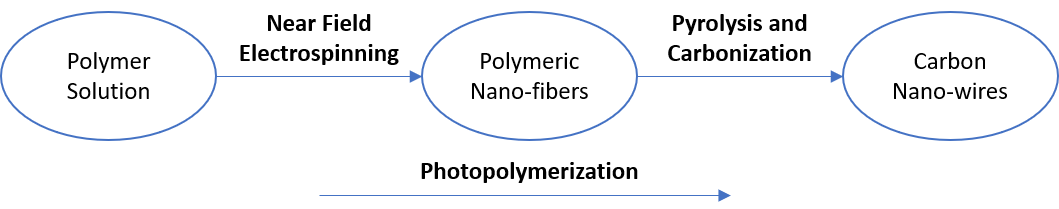
\includegraphics[width=0.95\textwidth]{./Figures/FabricationProcess.png}
%\decoRule
%\caption[Carbon Nano-wires Fabrication Process]{Fabrication process of carbon nano-wires to achieve through the proposed dissertation.}
%\label{fig:fabricationFlowChart}
%\end{figure}

%\begin{equation}
%\left(\tau _t^e-\frac{\tau _n^e \text{dr}}{\text{dz}}\right) 2 \pi  r+\frac{d \left(\pi  r^2
%   \left(\tau _{\text{zz}}-p\right)\right)}{\text{dz}}+\frac{\gamma  \text{dr} 2 \pi  r}{r
%   \text{dz}}+\rho  g \pi  r^2=\frac{d \left(\rho  \pi  r^2 v^2\right)}{\text{dz}}
%\label{eq:linearMomentum}
%\end{equation}